% ============================================================
% Chapter 26 --- Stokes' and Green's theorems
% Originally: content/week-11.tex, the three subsections \subsection{Sneak peek at Stokes'
%             theorem}, \subsection{Green's theorem and conservative fields} and
%             \subsection{The Poincare lemma and simply connected domains} (all promoted
%             to sections), followed by content/week-13.tex, \section{Stokes' theorem} and
%             \section{Area via Green's formula}. Corsin's order is preserved: the special
%             cases in week 11, the general theorem in week 13.
% ============================================================
\chapter{Stokes' and Green's Theorems}
\label{ch:stokes}

% Transition: Claude Opus 5 (Medium)
Everything in this part converges here. Stokes' theorem says that integrating $d\omega$ over a
submanifold is the same as integrating $\omega$ over its boundary --- one statement that
contains the fundamental theorem of calculus, Green's theorem, the divergence theorem and the
classical Stokes theorem as special cases. The chapter follows Corsin's own order: the special
cases first, where the content is visible, then the general theorem, then what it buys --- among
other things a formula computing an area from a boundary integral alone.

% Originally: content/week-11.tex, \subsection{Sneak peek at Stokes' theorem} --- promoted to a section

\section{Sneak peek at Stokes' theorem}
\label{sec:stokes_sneak_peek}

\begin{ainote}
Before the formal introduction of Stokes' theorem (\cref{sec:stokes_general}), Sascha presented introductory examples to build intuition. The classical version of Stokes' theorem states that for a surface $A \subset \mathbb{R}^3$ and a vector field $F$,
\[\int_A (\curl F)\cdot \nu \mathop{d\text{vol}}_2 = \int_{\partial A} F \cdot \tau \,dL,\]
where $\nu$ is the unit normal to $A$ and $\tau$ is the unit tangent vector to the boundary curve $\partial A$.
\end{ainote}

\begin{example}[Stokes' theorem on a hemisphere]
\label{ex:stokes_hemisphere}
Let $A := \{(x,y,z) \in \mathbb{R}^3 \mid x^2+y^2+z^2=1,\ z \geq 0\}$ be the upper hemisphere.
Given the vector field $F(x,y,z) := (z^2, x^2, y^2)\transp$, we can evaluate both sides of Stokes' theorem.
\begin{enumerate}[label=\textbf{\arabic*.}]
    \item \textbf{The rotation of $F$:} $\curl F = \nabla \times F = (2y, 2z, 2x)\transp$.
    \item \textbf{The surface normal:} On the unit sphere, the outward normal is simply $\nu(x,y,z) = (x,y,z)\transp$.
    \item \textbf{The boundary $\partial A$:} The boundary of the upper hemisphere is the unit circle in the $xy$-plane, $x^2+y^2=1$ with $z=0$. This can be parametrized by the closed path $\gamma : [0,2\pi] \to \mathbb{R}^3$,
    \[\gamma(t) = \begin{pmatrix} \cos t \\ \sin t \\ 0 \end{pmatrix}.\]
\end{enumerate}
Evaluating the path integral (the right-hand side of Stokes' theorem):
\[\int_{\partial A} F \cdot \tau \,dL = \int_0^{2\pi} F(\gamma(t)) \cdot \gamma'(t) \,dt.\]
Since $z=0$ on $\gamma$, we have $F(\gamma(t)) = (0, \cos^2 t, \sin^2 t)\transp$. The derivative is $\gamma'(t) = (-\sin t, \cos t, 0)\transp$.
\[\int_0^{2\pi} \begin{pmatrix} 0 \\ \cos^2 t \\ \sin^2 t \end{pmatrix} \cdot \begin{pmatrix} -\sin t \\ \cos t \\ 0 \end{pmatrix} dt = \int_0^{2\pi} \cos^3 t \,dt = 0.\]
\end{example}

\begin{example}[Path integral using Stokes' theorem]
\label{ex:stokes_path_integral}
Compute $\oint_\Gamma F \cdot \tau \,dL$ where $F(x,y,z) := (x, y, z)\transp$ and $\Gamma$ is the unit circle in the $xy$-plane (oriented counter-clockwise).

Instead of computing the line integral directly, we can use Stokes' theorem. The curve $\Gamma$ bounds the unit disk $A = \{(x,y,0) \mid x^2+y^2 \leq 1\}$.
First, we compute the rotation of $F$:
\[\curl F = \nabla \times F = \begin{pmatrix} \partial_y(z) - \partial_z(y) \\ \partial_z(x) - \partial_x(z) \\ \partial_x(y) - \partial_y(x) \end{pmatrix} = \begin{pmatrix} 0 \\ 0 \\ 0 \end{pmatrix}.\]
By Stokes' theorem, the line integral along $\Gamma$ bounds a surface $A$ on the sphere (for example, the upper hemisphere). The surface integral is:
\[\oint_\Gamma F \cdot \tau \,dL = \int_A (\curl F) \cdot \nu \mathop{d\text{vol}}_2 = 0.\]
\end{example}

% Supplement: Sascha Brack/Class Notes/Week_11_Notes_Monday.pdf, pp. 5--10

% Originally: content/week-11.tex, \subsection{Green's theorem and conservative fields} --- promoted to a section

\section{Green's theorem and conservative fields}
\label{sec:greens_theorem_conservative_fields}

\begin{ainote}
Green's theorem, conservative vector fields, and path integrals were also discussed in the Monday session. 
\end{ainote}

\begin{theorem}[Green's Theorem]
\label{thm:greens_theorem}
Let $F : U \to \mathbb{R}^2$ be a continuously differentiable vector field on an open set $U \subseteq \mathbb{R}^2$. Then, for any compact $C^1$ domain $\Omega \subseteq U$,
\[\int_\Omega \curl F \mathop{d\text{vol}}_2 = \int_{\partial\Omega} F \cdot \tau \,dL,\]
where $\tau$ is the unit tangent vector to the boundary $\partial\Omega$ oriented counter-clockwise (i.e.\ $\tau = (-\nu_2, \nu_1)\transp$, with $\nu$ being the outward unit normal).
\end{theorem}

\begin{ainote}
% Supplement: Sascha Brack/Class Notes/Week_10_Notes_Monday.pdf, p. 16
\begin{center}
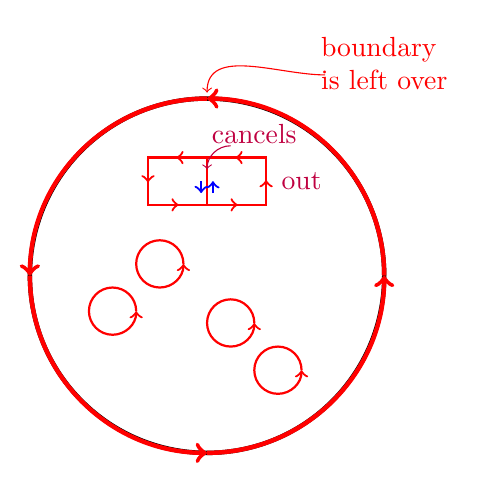
\begin{tikzpicture}[scale=1.5]
  % Domain
  \draw[ultra thick] (0,0) circle (1.5);
  % Boundary orientation
  \draw[red, ultra thick, ->] (1.5,0) arc (0:90:1.5);
  \draw[red, ultra thick, ->] (0,1.5) arc (90:180:1.5);
  \draw[red, ultra thick, ->] (-1.5,0) arc (180:270:1.5);
  \draw[red, ultra thick, ->] (0,-1.5) arc (270:360:1.5);
  
  \node[red, align=left] at (1.5, 1.8) {boundary\\is left over};
  \draw[red, ->] (1.0, 1.7) to[out=180, in=90] (0, 1.55);
  
  % Internal rotations
  \foreach \x/\y in {-0.6/-0.3, 0.4/-0.4, -0.2/0.1, 0.8/-0.8} {
    \draw[red, thick, ->] (\x,\y) arc (0:360:0.2);
  }
  
  % Two cancelling squares
  \draw[red, thick] (-0.5, 0.6) rectangle (0, 1.0);
  \draw[red, thick] (0, 0.6) rectangle (0.5, 1.0);
  % arrows
  \draw[red, thick, ->] (-0.25, 1.0) -- (-0.26, 1.0);
  \draw[red, thick, ->] (0.25, 1.0) -- (0.24, 1.0);
  \draw[red, thick, ->] (-0.5, 0.8) -- (-0.5, 0.79);
  \draw[red, thick, ->] (0.5, 0.8) -- (0.5, 0.81);
  \draw[red, thick, ->] (-0.25, 0.6) -- (-0.24, 0.6);
  \draw[red, thick, ->] (0.25, 0.6) -- (0.26, 0.6);
  
  \draw[blue, thick, ->] (-0.05, 0.8) -- (-0.05, 0.7);
  \draw[blue, thick, ->] (0.05, 0.7) -- (0.05, 0.8);
  
  \node[purple] at (0.4, 1.2) {cancels};
  \node[purple] at (0.8, 0.8) {out};
  \draw[purple, ->] (0.2, 1.1) to[out=180, in=90] (0, 0.9);
  
\end{tikzpicture}
\end{center}
We integrate the rotation inside the domain. Basically all the \qt{intermediate values} cancel out because for two points close to each other, the rotation points in opposite directions. Only the boundary is left over in the end!
\end{ainote}

\begin{example}[Area of a region via Green's theorem]
\label{ex:area_greens_theorem}
Consider a region $\Omega \subseteq \mathbb{R}^2$ defined by the region inside the curve $x^{2/3} + y^{2/3} = 1$ in the first quadrant, bounded by the axes. The curve can be parametrized as $\varphi(t) = (\cos^3 t, \sin^3 t)\transp$ for $t \in [0, \pi/2]$.

The area is $\vol_2(\Omega) = \int_\Omega 1 \mathop{d\text{vol}}_2$. We look for a vector field $F$ such that $\curl F = \partial_x F_2 - \partial_y F_1 \equiv 1$ on $\Omega$. A simple choice is $F(x,y) := (0, x)\transp$.
By Green's theorem, we have:
\[\vol_2(\Omega) = \int_\Omega \curl F \mathop{d\text{vol}}_2 = \int_{\partial\Omega} F \cdot \tau \,dL = \int_0^{\pi/2} F(\varphi(t)) \cdot \varphi'(t) \,dt.\]
Since $\tau(\varphi(t)) \,dL = \varphi'(t) \,dt$ along the parametrization, we compute the dot product:
\[F(\varphi(t)) \cdot \varphi'(t) = \begin{pmatrix} 0 \\ \varphi_1(t) \end{pmatrix} \cdot \begin{pmatrix} \varphi_1'(t) \\ \varphi_2'(t) \end{pmatrix} = \varphi_1(t)\varphi_2'(t).\]
This turns the area computation into a single 1D integral in $t$.
\end{example}

\begin{definition}[Conservative vector field]
\label{def:conservative_field}
Given a $C^k$ vector field $F$ on an open set $U \subseteq \mathbb{R}^n$, we call it \newterm{conservative} if there exists a scalar field $f : U \to \mathbb{R}$ of class $C^{k+1}$ such that $F \equiv \nabla f$. The function $f$ is called a \newterm{potential} for $F$.
\end{definition}

\begin{lemma}[Integrability conditions]
\label{lem:integrability_conditions}
Let $U \subseteq \mathbb{R}^n$ be open, and let $F$ be a $C^1$ conservative vector field on $U$ with components $F_1, \dots, F_n$. Then we necessarily have the integrability conditions:
\[\partial_j F_k = \partial_k F_j \qquad \text{for all } j, k \in \{1,\dots,n\}.\]
\end{lemma}
\begin{proof}
Let $f$ be a potential such that $F = \nabla f = (\partial_1 f, \dots, \partial_n f)\transp$. Then by Schwarz's theorem (symmetry of second derivatives),
\[\partial_j F_k = \partial_j(\partial_k f) = \partial_j\partial_k f = \partial_k\partial_j f = \partial_k(\partial_j f) = \partial_k F_j.\qedhere\]
\end{proof}

\begin{proposition}[Work along a path as difference of potential]
\label{prop:work_difference_potential}
Let $U \subseteq \mathbb{R}^n$ be open, and let $F : U \to \mathbb{R}^n$ be a continuous conservative vector field with potential $f$. Then for any $C^1$ path $\gamma : [0,1] \to U$, the line integral of $F$ along $\gamma$ depends only on the endpoints:
\[\int_\gamma F \cdot d\gamma = f(\gamma(1)) - f(\gamma(0)).\]
\end{proposition}
\begin{proof}
By definition of the path integral and the chain rule,
\begin{align*}
\int_\gamma F \cdot d\gamma &= \int_0^1 F(\gamma(t)) \cdot \gamma'(t) \,dt = \int_0^1 \nabla f(\gamma(t)) \cdot \gamma'(t) \,dt \\
&= \int_0^1 Jf(\gamma(t)) J\gamma(t) \,dt = \int_0^1 J(f \circ \gamma)(t) \,dt = \int_0^1 (f \circ \gamma)'(t) \,dt.
\end{align*}
By the fundamental theorem of calculus, this equals $(f \circ \gamma)(1) - (f \circ \gamma)(0) = f(\gamma(1)) - f(\gamma(0))$.
\end{proof}

\begin{example}[Line integral of a conservative field]
\label{ex:conservative_field_integral}
Consider the vector field $F : [0,1] \times [0,2] \to \mathbb{R}^2$ given by $F(x,y) := (y^2, 2xy)\transp$.
First, we show that $F$ is conservative by finding a potential $f$ such that $\nabla f = F$. We need $\partial_x f = y^2$ and $\partial_y f = 2xy$. Integrating the first equation with respect to $x$ gives $f(x,y) = xy^2 + c(y)$. Differentiating with respect to $y$ gives $\partial_y f = 2xy + c'(y)$, which must equal $2xy$. Thus $c'(y) = 0$, and we can choose $c(y) = 0$. The potential is $f(x,y) = xy^2$.

Now, let $\Gamma$ be a closed path on the boundary $\partial U$ of the domain, starting and ending at $\gamma(0) = \gamma(1) = (0,0)\transp$. By \cref{prop:work_difference_potential}, the line integral around this closed loop is simply the difference in potential at the endpoints:
\[\oint_\Gamma F \cdot d\gamma = f(\gamma(1)) - f(\gamma(0)) = f(0,0) - f(0,0) = 0.\]
\end{example}

% Originally: content/week-11.tex, \subsection{The Poincare lemma and simply connected domains} --- promoted

\section{The Poincaré lemma and simply connected domains}
\label{sec:poincare_lemma_simply_connected}

\begin{theorem}[Poincaré Lemma]
\label{thm:poincare_lemma}
Let $U \subseteq \mathbb{R}^n$ be open, and let $\alpha \in \Omega^1(U)$ be a $C^1$ closed $1$-form, that is, $d\alpha = 0$.
Let $\gamma_0, \gamma_1 : [0,1] \to U$ be piecewise $C^1$ paths with the same initial point $x_0$ and the same endpoint $x_1$. Suppose that $\gamma_0$ and $\gamma_1$ are \newterm{homotopic} in $U$ with fixed endpoints. For simplicity, assume that the homotopy $H : [0,1]^2 \to U$ is smooth. Then
\[\int_{\gamma_0} \alpha = \int_{\gamma_1} \alpha.\]
\end{theorem}

\begin{corollary}[Existence of potentials in simply connected domains]
\label{cor:potentials_simply_connected}
Let $U \subseteq \mathbb{R}^n$ be an open \newterm{simply connected} set. Then every closed $C^1$ $1$-form on $U$ is exact. That is, if $\alpha \in \Omega^1(U)$ satisfies $d\alpha = 0$, then there exists a function $f \in C^2(U)$ such that $\alpha = df$.
Equivalently, if $F \in C^1(U, \mathbb{R}^n)$ satisfies the integrability conditions
\[\partial_j F_k = \partial_k F_j \qquad \text{for all } j, k \in \{1,\dots,n\},\]
then $F$ is conservative: there exists a potential $f \in C^2(U)$ such that $\nabla f = F$.
\end{corollary}

\begin{ainote}[Intuition on simply connected spaces]
A space $U$ is simply connected if any closed loop in $U$ can be continuously contracted to a point within $U$ (i.e.\ any two paths with the same endpoints are homotopic). 

% Supplement: Sascha Brack/Class Notes/Week_12_Notes_Monday.pdf, p. 7
\begin{center}
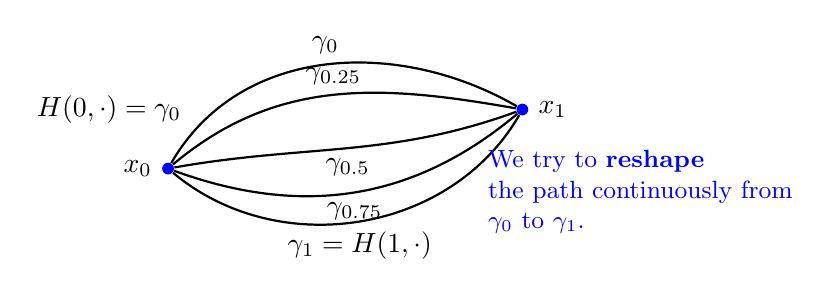
\begin{tikzpicture}[scale=1.5]
  \node[circle, fill=blue, inner sep=1.5pt, label=left:{$x_0$}] (x0) at (0,0) {};
  \node[circle, fill=blue, inner sep=1.5pt, label=right:{$x_1$}] (x1) at (3,0.5) {};
  
  \draw[thick] (x0) to[out=60, in=150] node[pos=0.5, above] {$\gamma_0$} (x1);
  \draw[thick] (x0) to[out=40, in=170] node[pos=0.5, above] {$\gamma_{0.25}$} (x1);
  \draw[thick] (x0) to[out=10, in=200] node[pos=0.5, below] {$\gamma_{0.5}$} (x1);
  \draw[thick] (x0) to[out=-20, in=220] node[pos=0.5, below] {$\gamma_{0.75}$} (x1);
  \draw[thick] (x0) to[out=-40, in=240] node[pos=0.5, below] {$\gamma_1 = H(1,\cdot)$} (x1);
  \node at (-0.5, 0.5) {$H(0,\cdot) = \gamma_0$};
  
  \node[blue, align=left, font=\small] at (4, -0.2) {We try to \textbf{reshape}\\the path continuously from\\$\gamma_0$ to $\gamma_1$.};
\end{tikzpicture}
\end{center}

Examples of simply connected spaces:
\begin{itemize}
    \item $\mathbb{R}^n$
    \item $\mathbb{R}^3 \setminus \{(0,0,0)\}$
\end{itemize}
Examples of spaces that are \emph{not} simply connected:
\begin{itemize}
    \item $S^1 \subseteq \mathbb{R}^2$ (the unit circle)
    \item $\mathbb{R}^3 \setminus \operatorname{span}\{(0,0,1)\transp\}$ (the $z$-axis removed)
    \item The torus
\end{itemize}
This topological property is what allows the integrability conditions to globally imply the existence of a potential.
\end{ainote}

% Supplement: Analysis_II_Script_v1.pdf, p. 153
\begin{example}[Integrability without a potential: why simple connectedness is needed]
\label{ex:vortex_field_not_conservative}
Let $U := \mathbb{R}^2\setminus\{0\}$ (which is \emph{not} simply connected, unlike its
$3$-dimensional analogue $\mathbb{R}^3\setminus\{0\}$ listed above) and
\[F(x,y) := \left(\frac{-y}{x^2+y^2},\ \frac{x}{x^2+y^2}\right), \qquad (x,y) \in U.\]
A direct computation gives
\[\partial_1F_2 = \partial_x\!\left(\frac{x}{x^2+y^2}\right) = \frac{-x^2+y^2}{(x^2+y^2)^2}
  = \partial_y\!\left(\frac{-y}{x^2+y^2}\right) = \partial_2F_1,\]
so $F$ satisfies the integrability conditions (\cref{lem:integrability_conditions})
\emph{everywhere} on $U$. Yet $F$ is not conservative: for the loop
$\gamma(t) := (\cos(2\pi t),\sin(2\pi t))$, $t\in[0,1]$, tracing the unit circle once
counterclockwise,
\[\oint_\gamma F\cdot d\gamma
  = 2\pi\int_0^1\langle(-\sin(2\pi t),\cos(2\pi t)),(-\sin(2\pi t),\cos(2\pi t))\rangle\,dt
  = 2\pi \neq 0,\]
which by \cref{prop:work_difference_potential} is impossible for a conservative field (a closed
loop would have to return $f(\gamma(1))-f(\gamma(0))=0$). This is exactly the witness that
\cref{cor:potentials_simply_connected} needs the hypothesis it has: the integrability
conditions are necessary but, on a domain that is not simply connected, not sufficient.
\end{example}

% Originally: content/week-13.tex, \section{Stokes' theorem} (Corsin Week 13)


\section{Stokes' theorem}
\label{sec:stokes_general}

% Source: Corsin Nick/Class Notes/Week 13.pdf, p. 2
\begin{theorem}[Stokes' theorem]
\label{thm:stokes_general}
Let $M \subseteq \mathbb{R}^n$ be an orientable $m$-manifold with (possibly empty) boundary,
and let $\omega \in \Omega^{m-1}(\mathbb{R}^n)$ have compact support in $\mathbb{R}^n$. Then
\[\int_{\partial M} \omega = \int_M d\omega.\]
\end{theorem}

\begin{ainote}
\Cref{thm:stokes_classical} was stated ahead of Corsin's own notes, as background
needed to solve \cref{ex:12.3}, in its classical $\mathbb{R}^3$ curl-theorem form. It is
exactly the case $m=2$, $n=3$, $\omega=\omega_F$ of the general theorem above, as
\cref{sec:stokes_in_r3} below confirms directly from Corsin's own derivation.
\end{ainote}

\subsection{Example: Green's theorem}
\label{sec:green_theorem_example}

% Source: Corsin Nick/Class Notes/Week 13.pdf, p. 2
\begin{example}[The exterior derivative of a $1$-form on $\mathbb{R}^2$]
\label{ex:exterior_derivative_r2}
Let $\omega(x,y) = P(x,y)\,dx + Q(x,y)\,dy$ be a $1$-form on $\mathbb{R}^2$. Then
\[
d\omega = dP\wedge dx + dQ\wedge dy = \left(\frac{\partial P}{\partial x}dx +
  \frac{\partial P}{\partial y}dy\right)\wedge dx + \left(\frac{\partial Q}{\partial x}dx +
  \frac{\partial Q}{\partial y}dy\right)\wedge dy = \left(\frac{\partial Q}{\partial x} -
  \frac{\partial P}{\partial y}\right) dx\wedge dy,
\]
using $dx\wedge dx = dy\wedge dy = 0$ and $dy\wedge dx = -dx\wedge dy$.
\end{example}

\subsection{Example: proof of Green's theorem}
\label{sec:green_theorem_proof}

% Source: Corsin Nick/Class Notes/Week 13.pdf, p. 3
\begin{ainote}
The theorem below is reproduced by Corsin directly from the lecture script (numbered there as
Theorem 14.24), as with the two definitions quoted in \cref{sec:orientable_manifolds}.
\end{ainote}

\begin{theorem}[Green's theorem in the plane]
\label{thm:green_theorem}
Let $F : U \to \mathbb{R}^2$ be a continuously differentiable vector field on an open set
$U \subseteq \mathbb{R}^2$. Then, for any compact $C^1$ domain $\Omega \subseteq U$,
\[\int_\Omega \curl F\,dx = \int_{\partial\Omega} F\cdot\tau\,dL,\]
with $\tau = \nu^\perp = (-\nu_2,\nu_1)$, where $\nu$ is the exterior unit normal.
\end{theorem}

Writing $F(x,y) = (P(x,y),Q(x,y))$, so that $\curl F = \partial_xQ - \partial_yP$ (the scalar
$2$-dimensional curl), \cref{thm:green_theorem} follows from
\cref{thm:stokes_general,ex:exterior_derivative_r2} applied to $\omega = P\,dx+Q\,dy$:
\[
\int_\Omega \curl F\,dx\,dy = \int_\Omega \left(\frac{\partial Q}{\partial x} -
  \frac{\partial P}{\partial y}\right) dx\wedge dy = \int_\Omega d\omega
  \overset{\text{Stokes}}{=} \int_{\partial\Omega} P(x,y)\,dx + Q(x,y)\,dy
  = \int_{\partial\Omega} F\cdot\tau\,dL.
\]

\begin{proof}[Justification of the last step]
Suppose $\gamma : [0,L] \to \partial\Omega$ is a $C^1$ curve of unit speed and positive
orientation, i.e.\ $\gamma'(t) = \tau(\gamma(t))$. Then
\[\langle F,\tau\rangle = \langle F,\gamma'(t)\rangle = (P\,dx+Q\,dy)(\gamma'(t)),\]
since $\tau = \begin{pmatrix}0&-1\\1&0\end{pmatrix}\nu$ is the tangent vector consistent with
the induced orientation, so integrating $(P\,dx+Q\,dy)(\gamma'(t))$ over $t \in [0,L]$ is
exactly $\int_{\partial\Omega} P\,dx+Q\,dy$ by \cref{def:integral_of_form_over_submanifold}.
\end{proof}

\subsection{Example: Stokes' theorem in \texorpdfstring{$\mathbb{R}^3$}{R\^{}3}}
\label{sec:stokes_in_r3}

% Source: Corsin Nick/Class Notes/Week 13.pdf, p. 4
Recall from \cref{ex:exterior_derivative_gradient_curl} that for $\omega_F =
\langle F,\cdot\rangle$, $d\omega_F = \langle\curl F,\cdot\times\cdot\rangle$. So, if $\Omega
\subseteq \mathbb{R}^3$ is a $2$-dimensional submanifold with boundary, parametrized by $\phi$
with tangent vectors $\tau_i := \partial_i\phi$ and exterior unit normal $\nu$, then
\[
\int_\Omega d\omega_F = \int_\Omega \langle\curl F,\tau_1\times\tau_2\rangle\,dx
  = \int_\Omega \langle\curl F,\nu\rangle\,d\vol_2 = \int_\Omega \vec\nabla\times\vec F\cdot
  d\vec A,
\]
and
\[\int_{\partial\Omega} \omega_F = \int_{\partial\Omega} \langle F,\tau\rangle\,d\vol_1
  = \int_{\partial\Omega} \vec F\cdot d\vec s.\]
By \cref{thm:stokes_general}, these are equal, which recovers \cref{thm:stokes_classical}.

% Source: Jérôme Paschoud/Notizen/Woche 13.1 Stokes.pdf, p. 4
\begin{theorem}[Stokes' theorem in 3D]
\label{thm:stokes_3d}
For an orientable, parametrized $2$-dimensional submanifold $M \subseteq \mathbb{R}^3$ with boundary $\partial M$, and a $C^1$ vector field $F$:
\[\int_M \curl(F) \cdot \nu \,d\vol_2 = \int_{\partial M} F \cdot \tau \,d\vol_1.\]
The orientation of $\partial M$ is chosen such that when traversing $\partial M$ in the direction of $\tau$, the surface $M$ (given by the normal $\nu$) is to the left (the ``right-hand rule'').
\end{theorem}

% Generator: Claude Opus 5 (High) --- FIG-26-03. This section is the chapter's main one and had
% no figure at all, while the theorem just above states its orientation convention purely in
% words. "The surface is to the left" is the one convention in this part of the course that a
% reader cannot reliably reconstruct from prose, and getting it backwards flips the sign of
% every answer, which is why it earns a picture here rather than a longer sentence.
%
% GEOMETRY, checked. The surface is a horizontal disc in the plane z = 0, drawn under the
% projection screen = (x, 0.4y + z), so a disc of radius 2 becomes an ellipse with semi-axes
% 2 and 0.8. The parametrization (2 cos t, 2 sin t, 0) maps to screen (2 cos t, 0.8 sin t),
% which runs right -> top -> left -> bottom as t increases, i.e. COUNTERCLOCKWISE on screen,
% and counterclockwise seen from +z is the sense that goes with the upward normal.
%
% The marked point is t = pi/2, the top of the ellipse, chosen because it is the only place
% where all three vectors are visually distinct:
%   tau     = d/dt (2 cos t, 2 sin t, 0) at t = pi/2, normalized  = (-1, 0, 0) -> LEFT on screen
%   nu      = (0, 0, 1)                                                        -> UP on screen
%   inward  = nu x tau = (0,0,1) x (-1,0,0) = (0, -1, 0)                       -> DOWN on screen
% The cross product is the content of the figure and is worth checking rather than trusting:
% (0,0,1) x (-1,0,0) = (0*0 - 1*0, 1*(-1) - 0*0, 0*0 - 0*(-1)) = (0,-1,0), and at the point
% (0,2,0) the direction (0,-1,0) does point back towards the centre, so it really is inward.
% Read that as the walker's rule: facing tau with nu upright, the left hand points along
% nu x tau, which is into M. At t = 0 this figure would be undrawable, since tau and nu would
% both project onto the same upward screen direction.
\begin{center}
\begin{tikzpicture}[>=Latex, scale=1.1]
  % The surface, and its boundary traversed counterclockwise on screen.
  \fill[MidnightBlue!7] (0,0) ellipse (2 and 0.8);
  \draw[MidnightBlue!70, thick] (0,0) ellipse (2 and 0.8);
  \foreach \a in {150,215,330} {
    \draw[MidnightBlue!70, very thick, ->]
      ({2*cos(\a-8)},{0.8*sin(\a-8)}) arc[start angle=\a-8, end angle=\a+8,
        x radius=2, y radius=0.8];
  }
  \node[MidnightBlue!70, font=\small] at (1.15,-0.30) {$M$};
  \node[MidnightBlue!70, font=\scriptsize, anchor=north] at (-1.62,-0.62) {$\partial M$};

  % The three directions at the top of the rim, where all three are distinguishable.
  \draw[OliveGreen, very thick, ->] (0,0.8) -- (0,1.85)
    node[anchor=south, font=\scriptsize] {$\nu$};
  \draw[BrickRed, very thick, ->] (0,0.8) -- (-1.05,0.8)
    node[anchor=south, font=\scriptsize] {$\tau$};
  % Anchored to the LEFT of the dashed arrow: anchored to its right it came to rest just before
  % the "$M$" label inside the ellipse, and the two read as one string, "into M M".
  \draw[gray!50!black, thick, dashed, ->] (0,0.8) -- (0,0.12)
    node[anchor=north east, font=\scriptsize, text=gray!45!black] {into $M$};
  \fill[MidnightBlue!70] (0,0.8) circle (1.5pt);

  \node[font=\scriptsize, anchor=north, align=center] at (0,-1.15)
    {walking along $\tau$ with $\nu$ upright, $M$ lies to the left:\\
     the leftward direction is $\nu\times\tau$};
\end{tikzpicture}
\end{center}

\begin{remark}[The convention as a formula]
\label{rem:right_hand_rule_as_cross_product}
\qt{To the left} is a reliable instruction only once one knows which way is up, and $\nu$ is what
supplies that. The picture above turns the sentence into an identity that can be checked instead
of visualised: at a boundary point, the direction pointing from $\partial M$ into $M$ is
\[\text{inward} = \nu\times\tau.\]
Equivalently $\tau = \text{inward}\times\nu$, so any two of the three determine the third. On the
unit disc in the $xy$-plane with $\nu = e_3$, at the point $(1,0,0)$, the positively oriented
$\tau$ is $(0,1,0)$ and $\nu\times\tau = (-1,0,0)$ does point at the origin, confirming the
familiar counterclockwise convention.

Reversing $\nu$ reverses $\tau$, which is why both sides of \cref{thm:stokes_3d} change sign
together and the theorem is insensitive to the choice. What it is \emph{not} insensitive to is
choosing the two independently, and that is the error the formula above rules out.
\end{remark}

\begin{example}[Stokes' theorem on a hemisphere]
\label{ex:stokes_hemisphere_linear_field}
% Michael's Bsp. 20.1.2
Let $F(x,y,z) := (z, x, y)\transp$. We want to compute the flux of the curl of $F$ through the upper hemisphere $H := \{(x,y,z) \in \mathbb{R}^3 \mid x^2 + y^2 + z^2 = 1,\ z \geq 0\}$.

First, the curl of $F$ is:
\[\curl(F) = \begin{pmatrix} \partial_y F_3 - \partial_z F_2 \\ \partial_z F_1 - \partial_x F_3 \\ \partial_x F_2 - \partial_y F_1 \end{pmatrix} = \begin{pmatrix} 1 - 0 \\ 1 - 0 \\ 1 - 0 \end{pmatrix} = \begin{pmatrix} 1 \\ 1 \\ 1 \end{pmatrix}.\]
By \cref{thm:stokes_3d}, the flux of $\curl(F)$ through $H$ equals the line integral of $F$ along the boundary $\partial H$. The boundary is the unit circle in the $xy$-plane, which we parametrize by $\gamma(t) = (\cos t, \sin t, 0)\transp$ for $t \in [0, 2\pi]$. The tangent vector is $\gamma'(t) = (-\sin t, \cos t, 0)\transp$.
The line integral is:
\begin{align*}
\int_{\partial H} F \cdot d\gamma &= \int_0^{2\pi} F(\gamma(t)) \cdot \gamma'(t) \,dt \\
&= \int_0^{2\pi} \begin{pmatrix} 0 \\ \cos t \\ \sin t \end{pmatrix} \cdot \begin{pmatrix} -\sin t \\ \cos t \\ 0 \end{pmatrix} \,dt \\
&= \int_0^{2\pi} \cos^2 t \,dt = \pi.
\end{align*}
Thus, $\int_H \curl(F) \cdot \nu \,d\vol_2 = \pi$.
\end{example}

% Supplement: Analysis_II_Script_v1.pdf, p. 163
\begin{exercise}[Flux through a cylinder, direct and via Stokes]
\label{ex:cylinder_flux_direct_and_stokes}
Let $F(x,y,z) := (yz,x^2,1)\transp$ on $\mathbb{R}^3$, and let $M$ be the lateral surface of the
cylinder $M := \{(x,y,z) : x^2+y^2=1,\ 0<z<1\}$, with the outward-pointing normal
$\nu(x,y,z)=(x,y,0)$. Compute $\int_M\curl(F)\cdot\nu\,d\vol_2$ directly, and again using
Stokes' theorem.
\end{exercise}

\begin{exercisesolution}[Proof of \cref{ex:cylinder_flux_direct_and_stokes}]
% Generator: Claude Sonnet 5 (High)
First, $\curl(F) = (\partial_yF_3-\partial_zF_2,\ \partial_zF_1-\partial_xF_3,\
\partial_xF_2-\partial_yF_1) = (0,\ y,\ 2x-z)$.

\textbf{Directly.} Parametrize $M$ by $\phi(\theta,z) := (\cos\theta,\sin\theta,z)$,
$(\theta,z)\in[0,2\pi)\times(0,1)$; then
$\partial_\theta\phi\times\partial_z\phi = (\cos\theta,\sin\theta,0) = \nu(\phi(\theta,z))$,
already a unit vector, so $d\vol_2 = d\theta\,dz$. Then
$\curl(F)(\phi(\theta,z)) = (0,\sin\theta,2\cos\theta-z)$, and
\[\int_M\curl(F)\cdot\nu\,d\vol_2 = \int_0^1\!\int_0^{2\pi}
  \big\langle(0,\sin\theta,2\cos\theta-z),(\cos\theta,\sin\theta,0)\big\rangle\,d\theta\,dz
  = \int_0^1\!\int_0^{2\pi}\sin^2\theta\,d\theta\,dz = \pi.\]

\textbf{Via Stokes.} The boundary $\partial M$ consists of the two circles $z=0$ and $z=1$; the
orientation induced by the outward normal $\nu$ (right-hand rule) traverses the \emph{bottom}
circle ($z=0$) with $\theta$ increasing and the \emph{top} circle ($z=1$) with $\theta$
\emph{decreasing}. The parameter rectangle $[0,2\pi]\times[0,1]$ has $z=0$ as part of its
positively-oriented boundary traversed left to right and $z=1$ traversed right to left, and the
two vertical edges $\theta=0,2\pi$ cancel since they are the same curve in $M$. This is the
phenomenon drawn in \cref{sec:submanifolds_with_boundary}: one consistently oriented cylinder
induces senses on its two rims that turn opposite ways when both are viewed from the same side,
and \cref{rem:cylinder_opposite_boundary_senses} explains why that is the convention working
rather than failing. With
$\gamma_0(\theta):=(\cos\theta,\sin\theta,0)$ and $\gamma_1(\theta):=(\cos\theta,\sin\theta,1)$,
both for $\theta\in[0,2\pi]$,
\[F(\gamma_0(\theta)) = (0,\cos^2\theta,1), \qquad F(\gamma_1(\theta)) = (\sin\theta,\cos^2\theta,1),\]
and $\gamma_0'(\theta)=\gamma_1'(\theta)=(-\sin\theta,\cos\theta,0)$, so
\[\int_0^{2\pi} F(\gamma_0(\theta))\cdot\gamma_0'(\theta)\,d\theta = \int_0^{2\pi}\cos^3\theta\,d\theta = 0,\]
\[\int_0^{2\pi} F(\gamma_1(\theta))\cdot\gamma_1'(\theta)\,d\theta
  = \int_0^{2\pi}\big({-}\sin^2\theta+\cos^3\theta\big)\,d\theta = -\pi.\]
The bottom circle is traversed with $\theta$ increasing (contributing $+0$) and the top circle
with $\theta$ \emph{decreasing} (contributing $-({-}\pi) = \pi$), so
$\int_{\partial M}F\cdot\tau\,d\vol_1 = 0+\pi = \pi$, agreeing with the direct computation.
\end{exercisesolution}

% Supplement: Analysis_II_Script_v1.pdf, p. 163
\begin{exercise}[Flux through a spherical cap, via Stokes and via Gauss]
\label{ex:spherical_cap_flux_stokes_gauss}
Let $0<h<1$ and let $S := \{(x,y,z)\in S^2 : z>-h\}$ be the part of the unit sphere above
height $-h$. Consider $F(x,y,z) := (-y,x,0)\transp$. Calculate the flux
$\int_S\curl(F)\cdot\nu\,d\vol_2$ (outward normal) directly, once using Stokes' theorem, and
once using the divergence theorem.
\end{exercise}

\begin{exercisesolution}[Proof of \cref{ex:spherical_cap_flux_stokes_gauss}]
% Generator: Claude Sonnet 5 (High)
Here $\curl(F) = (0,0,2)$, a constant field, and on $S^2$ the outward normal is
$\nu(x,y,z)=(x,y,z)$ itself, so $\langle\curl(F),\nu\rangle = 2z$.

\textbf{Directly.} Using colatitude $\varphi\in[0,\arccos(-h)]$ (so $z=\cos\varphi>-h$) and
$d\vol_2=\sin\varphi\,d\varphi\,d\theta$,
\[\int_S 2z\,d\vol_2 = \int_0^{2\pi}\!\int_0^{\arccos(-h)} 2\cos\varphi\sin\varphi\,d\varphi\,d\theta
  = 2\pi\Big[{-}\tfrac12\cos(2\varphi)\Big]_0^{\arccos(-h)} = 2\pi(1-h^2),\]
using $\cos(2\arccos(-h)) = 2h^2-1$.

\textbf{Via Stokes.} $\partial S$ is the circle $x^2+y^2=1-h^2$, $z=-h$, of radius
$r:=\sqrt{1-h^2}$, oriented (right-hand rule, outward normal) by
$\gamma(\theta) := (r\cos\theta,r\sin\theta,-h)$, $\theta\in[0,2\pi]$. Then
$\gamma'(\theta) = (-r\sin\theta,r\cos\theta,0)$ and $F(\gamma(\theta)) =
(-r\sin\theta,r\cos\theta,0)$, so
\[\int_{\partial S}F\cdot d\gamma = \int_0^{2\pi}\big(r^2\sin^2\theta+r^2\cos^2\theta\big)\,d\theta
  = 2\pi r^2 = 2\pi(1-h^2),\]
agreeing with the direct computation.

\textbf{Via Gauss.} Since $\divg(\curl F)\equiv0$ (\cref{ex:curl_grad_div_curl_zero}), the flux
of $\curl(F)$ through any surface with boundary $\partial S$ is the same. Replace $S$ by the
flat disk $D := \{x^2+y^2\leq1-h^2,\ z=-h\}$, with upward normal $(0,0,1)$: $S\cup(-D)$
(the cap together with the disk, reversed) bounds the solid cap $\Omega$, and the divergence
theorem gives $\int_S\curl(F)\cdot\nu\,d\vol_2 - \int_D\curl(F)\cdot(0,0,1)\,d\vol_2 =
\int_\Omega\divg(\curl F)\,d\vol_3 = 0$. Since $\langle\curl F,(0,0,1)\rangle\equiv2$,
\[\int_S\curl(F)\cdot\nu\,d\vol_2 = \int_D 2\,d\vol_2 = 2\cdot\vol_2(D) = 2\pi(1-h^2),\]
the area of a disk of radius $\sqrt{1-h^2}$ times $2$, again the same answer.
\end{exercisesolution}

% Generator: Claude Sonnet 5 (High) --- new content, tying together four theorems this document
% proves separately (FTC-via-Gauss in \cref{sec:gauss_intuition}, Green in
% \cref{sec:green_theorem_proof}, classical Stokes in \cref{sec:stokes_in_r3}, and the
% divergence theorem in \cref{sec:flux_divergence_theorem}) as one theorem, stated once, here.
\begin{remark}[One theorem, four costumes]
\label{rem:one_theorem_four_costumes}
Every integral theorem proved in this part of the course is the single identity
$\int_M d\omega = \int_{\partial M}\omega$ of \cref{thm:stokes_general}, for a different choice
of the dimension $m$ of $M$ and the degree of $\omega$. Collected in one place:
\begin{center}
\small
\begin{tabular}{@{}lllll@{}}
\toprule
\textbf{Theorem} & $M$ & $m$ & $\omega$ & $d\omega$ \\
\midrule
FTC &
  $[a,b]\subset\mathbb{R}$ & $1$ & $f$ ($0$-form) & $f'\,dx$ \\
Green (\cref{thm:green_theorem}) &
  $\Omega\subseteq\mathbb{R}^2$ & $2$ & $P\,dx+Q\,dy$ & $(\partial_xQ{-}\partial_yP)\,dx\!\wedge\! dy$ \\
Classical Stokes (\cref{thm:stokes_classical}) &
  surface $S\subset\mathbb{R}^3$ & $2$ & $\omega_F$ & $\omega_{\curl F}^2$ \\
Divergence (\cref{thm:gauss_divergence}) &
  $\Omega\subseteq\mathbb{R}^n$ & $n$ & $\omega_F^{n-1}$ & $(\divg F)\,dx^1\!\wedge\!\cdots\!\wedge\! dx^n$ \\
\bottomrule
\end{tabular}
\end{center}
Each row's $\int_M d\omega = \int_{\partial M}\omega$ reads off as exactly that row's theorem.
The top row is \cref{sec:gauss_intuition}'s $n=1$ computation seen from the other side: there,
$f$ played the role of a $1$-dimensional vector field and the identity was reached via the
divergence theorem; here $f$ is instead a $0$-form and the same identity is the $m=1$ case of
\cref{thm:stokes_general} directly. These are two routes to the same fact, matching
\cref{ex:exterior_derivative_gradient_curl}'s remark that $df = \langle\nabla f,\cdot\rangle$ is
exactly the shape that makes this specialization work. The bottom row uses
$d\omega_F^{n-1} = (\divg F)\,dx^1\wedge\cdots\wedge dx^n$
(\cref{ex:exterior_derivative_gradient_curl}, item 3) together with the identification of
$\int_{\partial\Omega}\omega_F^{n-1}$ with the flux $\int_{\partial\Omega}\langle
F,\nu\rangle\,d\vol_{n-1}$ already noted in \cref{ch:pullbacks}.

The pattern is worth stating in words, because it is easy to lose under the notation: a
$k$-dimensional derivative measured \emph{inside} a region always equals the corresponding
$(k{-}1)$-dimensional quantity measured on its \emph{boundary}. Differentiation and taking a
boundary are, in this precise sense, the same operation viewed from two sides. That is also
exactly the content of $d^2=0$ (\cref{thm:exterior_derivative}\textbf{(3)}): a boundary has no
boundary, just as $d\omega$ has no further exterior derivative to take that isn't already zero.
\end{remark}

% Source: old_exams/examFS24.pdf (21 August 2024), Problem 3, parts 1--2, p. 10
% Extractor: Gemini 3.6 Flash (High)
% Correction: Claude Opus 5 (High) --- \operatorname{rot} -> \curl and J\Phi -> \Jac\Phi per the
% declared-macro rule; \iint -> \int, matching thm:green_theorem two pages above.
\begin{exercise}[Curl identity and Green's formula area preservation]
\label{ex:curl_identity_greens_formula}
Let $\Omega \subseteq \mathbb{R}^2$ be a bounded $C^1$ domain, and let $\Phi = (\Phi_1, \Phi_2) \in C^2(\overline{\Omega}, \mathbb{R}^2)$ be a vector-valued mapping, not assumed to be a diffeomorphism.
\begin{enumerate}[label=\textbf{(\alph*)}]
  \item Consider the vector field $V \in C^1(\overline{\Omega}, \mathbb{R}^2)$ defined by
  \[V := (\Phi_1 \partial_1 \Phi_2, \Phi_1 \partial_2 \Phi_2)\transp = \Phi_1 \nabla \Phi_2.\]
  Prove that $\curl V(x) = \det \Jac\Phi(x)$ for all $x \in \overline{\Omega}$.
  \item Let $\Psi \in C^2(\overline{\Omega}, \mathbb{R}^2)$ be another mapping such that $\Phi(x) = \Psi(x)$ for all $x \in \partial \Omega$. Prove that
  \[\int_\Omega \det \Jac\Phi(x) \, dx = \int_\Omega \det \Jac\Psi(x) \, dx.\]
\end{enumerate}
\exhint[Official hint]{Use Green's formula (i.e.\ 2D Stokes) on the plane.}
\exinfo{This exercise is taken from the exam of 21 August 2024, Problem 3. The original continues
with four further parts about $\Phi(\overline{B_1})$ when $\Phi$ fixes the unit circle.}
\end{exercise}


% Originally: content/week-13.tex, \section{Area via Green's formula} (Corsin Week 13)

\section{Area via Green's formula}
\label{sec:area_via_green}

% Source: Corsin Nick/Class Notes/Week 13.pdf, pp. 5--6
% Kept inline: solved directly in Corsin Nick/Class Notes/Week 13.pdf, pp. 5--6.
\begin{exercise}[Area as a boundary functional]
\label{ex:area_boundary_functional}
Suppose $\gamma : [0,L) \to \mathbb{R}^2$ traces the boundary of a connected $C^\infty$-domain
$U \subseteq \mathbb{R}^2$ in the positive direction. Express the area of $U$ as a functional
of $\gamma$.
\end{exercise}

\begin{exercisesolution}
By definition, $A(U) = \int_U dx\,dy = \int_U 1\,dx\wedge dy$. By Green's formula
(\cref{thm:green_theorem}, in its $1$-form guise $\int_\Omega d\omega =
\int_{\partial\Omega}\omega$),
\[\int_U 1\,dx\wedge dy = \int_0^L \langle F\circ\gamma(t),\gamma'(t)\rangle\,dt\]
for any $F : \overline U \to \mathbb{R}^2$ satisfying $\partial_xF^2 - \partial_yF^1 = 1$. This
is satisfied by $F(x,y) = \tfrac12(-y,x)$, giving the \newterm{shoelace formula}
(\germanterm{Gau\ss sche Trapezformel})
\[A(\gamma) = \frac12\int_0^L \big[\gamma_1(t)\gamma_2'(t) - \gamma_2(t)\gamma_1'(t)\big]\,dt.\]
\end{exercisesolution}

\begin{example}[Ellipse]
\label{ex:area_ellipse}
The path $\gamma : [0,2\pi) \to \mathbb{R}^2$, $t \mapsto (a\cos t,b\sin t)$, traces the
boundary of an ellipse. By \cref{ex:area_boundary_functional},
\[
A(\gamma) = \frac12\int_0^{2\pi} \big[a\cos t\cdot b\cos t - b\sin t\cdot(-a\sin t)\big]\,dt
  = \frac{ab}{2}\int_0^{2\pi} dt = \pi ab.
\]
For the circle $a=b=:r$, this gives the familiar $A = \pi r^2$.
\end{example}

\begin{ainote}
Corsin adds, in the same breath as the ellipse's area: \qt{Famously, there exists no closed
form solution for the length of the boundary of an ellipse} --- the ellipse's perimeter is a
complete elliptic integral of the second kind, not an elementary function, unlike its area.
\end{ainote}


% --- exercises relocated here from the dissolved sheets ---

% Originally: content/week-12.tex, \exercisesheet{12}, problem 12.3
% Source: exercises/Ex12_Analysis2_eng.pdf

\begin{exercise}[12.3 --- Work along paths and Stokes \textnormal{(important)}]
\label{ex:12.3}
Let $F : \mathbb{R}^3 \setminus (\{(0,0)\}\times\mathbb{R}) \to \mathbb{R}^3$ be the vector
field defined by
\[F(x,y,z) = \left(\frac{2(xz+y)}{x^2+y^2},\ \frac{2(yz-x)}{x^2+y^2},\ \log(x^2+y^2)\right)\]
and let $\gamma_1,\gamma_2,\gamma_3 : [0,2\pi] \to \mathbb{R}^3$ be the paths
\[\gamma_1(t) = (\cos t,\sin t,0), \qquad \gamma_2(t) = (2\cos t,2\sin t,2), \qquad
  \gamma_3(t) = (3\cos t+6,3\sin t,3).\]
\begin{enumerate}[label=\textbf{\arabic*.}]
  \item Describe the domain of definition of $F$. Is it connected? Is it simply connected?
  \item Compute the rotation $\curl(F)$ of $F$ and the path integral $\int_{\gamma_1} F\cdot
  d\gamma_1$ of $F$ along $\gamma_1$. Is $F$ conservative?
  \item Explain how the equation $\int_{\gamma_1} F\cdot d\gamma_1 = \int_{\gamma_2} F\cdot
  d\gamma_2$ follows from Stokes' theorem.
  \item Does Stokes' theorem imply that $\int_{\gamma_1} F\cdot d\gamma_1 = \int_{\gamma_3}
  F\cdot d\gamma_3$ holds?
\end{enumerate}
\end{exercise}

% Source: exercises/Ex12_Analysis2_eng.pdf, p. 2

% Originally: content/week-12.tex, \exercisesheet{12}, problem 12.4
% Source: exercises/Ex12_Analysis2_eng.pdf

\begin{exercise}[12.4 --- True or False \textnormal{(important)}]
\label{ex:12.4}
Let $U := \mathbb{R}^3\setminus\{0\}$ and $F \in C^1(U,\mathbb{R}^3)$. For $r>0$ set
\[I_r := \int_{\partial B_r} \langle F,n\rangle\,dS\]
where $n$ denotes the outward normal. Which of the following statements are always true?
\begin{enumerate}[label=\textbf{(\alph*)}]
  \item If $F$ is divergence-free, then $I_r=0$ for all $r>0$.
  \item If $F$ is divergence-free, then the value of $I_r$ does not depend on $r$.
  \item If $F$ is curl-free, then the value of $I_r$ does not depend on $r$.
  \item If $F = \curl(G)$ for a vector field $G \in C^1(U,\mathbb{R}^3)$ and $\lvert F(x)
  \rvert \leq C/\lvert x\rvert$, then $I_r=0$ for all $r>0$.
\end{enumerate}
\end{exercise}

% Source: exercises/Ex12_Analysis2_eng.pdf, p. 2

% Originally: content/week-12.tex, \exercisesheet{12}, problem 12.5
% Source: exercises/Ex12_Analysis2_eng.pdf

\begin{exercise}[12.5 --- Conservative vector fields \textnormal{(important)}]
\label{ex:12.5}
For which values of $\lambda \in \mathbb{R}$ is the vector field $F : \mathbb{R}^2 \to
\mathbb{R}^2$ defined by
\[F(x,y) = \begin{pmatrix} \lambda x e^y \\ (y+1+x^2)e^y \end{pmatrix}\]
conservative? Determine a potential for $F$ for these values.
\end{exercise}

% Source: exercises/Ex12_Analysis2_eng.pdf, p. 3

% Originally: content/week-12.tex, \exercisesheet{12}, problem 12.8
% Source: exercises/Ex12_Analysis2_eng.pdf

\begin{exercise}[12.8 --- Multiple Choice \textnormal{(important)}]
\label{ex:12.8}
Let $Q = [a,b]\times[c,d] \subseteq \mathbb{R}^2$ and $f \in C(Q,\mathbb{R}^2)$. Let $n$ be an
outward normal field on $Q$ and
\[I_b = \int_{[a,b]\times\{c\}} \langle f,n\rangle, \qquad I_t = \int_{[a,b]\times\{d\}}
  \langle f,n\rangle, \qquad I_l = \int_{\{a\}\times[c,d]} \langle f,n\rangle, \qquad
  I_r = \int_{\{b\}\times[c,d]} \langle f,n\rangle.\]
Which of the following expressions corresponds to the outer flux of $f$ through $\partial Q$?
\begin{enumerate}[label=\textbf{(\alph*)}]
  \item $I_b - I_t + I_r - I_l$
  \item $I_b + I_t + I_r + I_l$
  \item $I_b + I_t - I_r - I_l$
  \item $-I_b + I_t - I_r + I_l$
\end{enumerate}
\end{exercise}

% Source: exercises/Ex12_Analysis2_eng.pdf, p. 3

% Originally: content/week-12.tex, \section{Solutions}

\section{Solutions}
\label{sec:stokes_solutions}

\begin{exercisesolution}[Solution of \cref{ex:12.3}]
\textbf{1.} The domain is $\{(x,y,z) \in \mathbb{R}^3 : (x,y) \neq (0,0)\}$, i.e.\
$\mathbb{R}^3$ with the $z$-axis removed. It is connected (path-connected: any two points can
be joined by a path avoiding the axis), but not simply connected: $\gamma_1$, for instance, which
winds once around the axis, cannot be contracted to a point without crossing it. (It is also
not convex: the segment from $(-1,0,0)$ to $(1,0,0)$ leaves the domain.)

\textbf{2.} Writing $F = (F^1,F^2,F^3)$ with $F^1 = 2(xz+y)/(x^2+y^2)$, $F^2 =
2(yz-x)/(x^2+y^2)$, $F^3 = \log(x^2+y^2)$, a direct computation of each pair of mixed
partials gives
\[\partial_y F^3 = \partial_z F^2 = \frac{2y}{x^2+y^2}, \qquad
  \partial_z F^1 = \partial_x F^3 = \frac{2x}{x^2+y^2}, \qquad
  \partial_x F^2 = \partial_y F^1 = \frac{2(x^2-y^2-2xyz)}{(x^2+y^2)^2},\]
so $\curl F = (\partial_yF^3-\partial_zF^2,\ \partial_zF^1-\partial_xF^3,\ \partial_xF^2-
\partial_yF^1) = (0,0,0)$: $F$ is curl-free. On $\gamma_1$, $x=\cos t$, $y=\sin t$, $z=0$,
$x^2+y^2=1$, so $F(\gamma_1(t)) = (2\sin t,\,-2\cos t,\,0)$ and $\gamma_1'(t) = (-\sin t,
\cos t,0)$, giving
\[\int_{\gamma_1} F\cdot d\gamma_1 = \int_0^{2\pi} \big(2\sin t\cdot(-\sin t) + (-2\cos t)
  \cdot\cos t\big)\,dt = \int_0^{2\pi} -2\,dt = -4\pi.\]
Since this is nonzero on a closed loop, $F$ is \textbf{not} conservative. It is curl-free, but
its domain is not simply connected (part 1), so curl-free does not force conservative here.

\textbf{3.} Let $S := \{(x,y,z) : \sqrt{x^2+y^2} = 1+z/2,\ 0\leq z\leq2\}$, the cone swept out
by linearly interpolating the radius from $\gamma_1$ ($z=0$, radius $1$) to $\gamma_2$ ($z=2$,
radius $2$), parametrized by $H(s,t) := \big((1+s)\cos t,(1+s)\sin t,2s\big)$ for $(s,t) \in
[0,1]\times[0,2\pi]$. Since the radius $1+s \geq 1 > 0$ throughout, $S$ never meets the
$z$-axis and lies entirely in the domain of $F$; its oriented boundary (outward normal) is
$\gamma_2$ minus $\gamma_1$. Since $\curl F = 0$ on $S$ by part 2, \cref{thm:stokes_classical}
gives
\[\int_{\gamma_2} F\cdot d\gamma_2 - \int_{\gamma_1} F\cdot d\gamma_1 = \int_{\partial S}
  F\cdot ds = \int_S \curl F\cdot d\vec n = 0,\]
i.e.\ $\int_{\gamma_1} F\cdot d\gamma_1 = \int_{\gamma_2} F\cdot d\gamma_2$.

\textbf{4.} No. The disk $D := \{(x,y,z) : (x-6)^2+y^2 \leq 9,\ z=3\}$, oriented upward, has
oriented boundary exactly $\gamma_3$, and $D$ lies entirely in the domain of $F$ (it does not
meet the $z$-axis, since its center $(6,0,3)$ is at distance $6$ from the axis and its radius
is only $3$). By \cref{thm:stokes_classical} with $\curl F=0$,
\[\int_{\gamma_3} F\cdot d\gamma_3 = \int_{\partial D} F\cdot ds = \int_D \curl F\cdot d\vec n
  = 0.\]
Since $\int_{\gamma_1} F\cdot d\gamma_1 = -4\pi \neq 0 = \int_{\gamma_3} F\cdot d\gamma_3$, the
two do \emph{not} agree, and Stokes' theorem gives no reason to expect they would: unlike the
pair $(\gamma_1,\gamma_2)$, there is no surface joining $\gamma_1$ and $\gamma_3$ that stays
inside the domain, since $\gamma_1$ winds around the excluded axis and $\gamma_3$ does not.
\end{exercisesolution}

% Verified: solved independently, all four parts match Sol12_Analysis2_eng.pdf exactly.
% Note: the official solution's part 2 labels vanishing curl as "divergence-free" where it
% visibly means curl-free (computes curl F, not div F) --- a wording slip, not repeated here.

\begin{exercisesolution}[Solution of \cref{ex:12.4}]
\textbf{(a) False.} The Newton potential's gradient $F(x) = \nabla(1/\lvert x\rvert) =
-x\lvert x\rvert^{-3}$ is divergence-free on $U$ (it is $V_{-3}$ up to sign, from
\cref{ex:11.5}, with $n=3$), yet $I_r = \int_{\partial B_r} F\cdot n\,dS =
-\vol_2(\partial B_r) \neq 0$.

\textbf{(b) True.} Applying \cref{thm:gauss_divergence} on the shell $B_{r_2}\setminus
B_{r_1} \Subset U$ for $0<r_1<r_2$, whose boundary is $\partial B_{r_2}$ (outward) together
with $\partial B_{r_1}$ with reversed orientation,
\[0 = \int_{B_{r_2}\setminus B_{r_1}} \divg F\,dx = I_{r_2} - I_{r_1},\]
so $I_r$ is independent of $r$.

\textbf{(c) False.} Take $F(x) = x = \tfrac12\nabla\lvert x\rvert^2$, which is curl-free
(being a gradient). Then $\divg F \equiv 3$, so by \cref{thm:gauss_divergence}, $I_r =
\int_{B_r} 3\,dx = 3\vol_3(B_r) = 4\pi r^3$, which depends on $r$.

\textbf{(d) True.} If $F = \curl G$ then $\divg F = \divg(\curl G) = 0$ (a standard vector
identity), so part (b) applies and $I_r$ is independent of $r$. On the other hand,
\[\lvert I_r\rvert \leq \int_{\partial B_r} \lvert\langle F,n\rangle\rvert\,dS \leq
  \frac{C}{r}\,\vol_2(\partial B_r) = \frac{C}{r}\cdot4\pi r^2 = 4\pi C r \longrightarrow 0
  \quad\text{as } r\to0^+.\]
Since $I_r$ is constant in $r$ and this constant is a limit of values tending to $0$, $I_r=0$
for all $r>0$.
\end{exercisesolution}

% Verified: solved independently, all four parts match Sol12_Analysis2_eng.pdf.

\begin{exercisesolution}[Solution of \cref{ex:12.5}]
Writing $F = (F^1,F^2)$ with $F^1 = \lambda xe^y$, $F^2 = (y+1+x^2)e^y$, the integrability
condition is $\partial_yF^1 = \partial_xF^2$:
\[\partial_yF^1 = \lambda xe^y, \qquad \partial_xF^2 = 2xe^y.\]
Since $\mathbb{R}^2$ is convex (so integrability is equivalent to conservativity here), $F$
is conservative if and only if $\lambda=2$.

For $\lambda=2$, seek $f$ with $\partial_xf = F^1 = 2xe^y$: integrating in $x$,
$f(x,y) = x^2e^y + g(y)$ for some function $g$. Then $\partial_yf = x^2e^y+g'(y)$ must equal
$F^2 = (y+1+x^2)e^y$, so $g'(y) = (y+1)e^y$; integrating by parts, $\int(y+1)e^y\,dy =
ye^y - e^y + e^y = ye^y$ (up to an additive constant). Hence
\[f(x,y) = \boxed{\ (x^2+y)e^y\ } \qquad (\text{unique up to an additive constant}),\]
which one checks directly satisfies $\nabla f = F$.
\end{exercisesolution}

% Verified: solved independently, lambda=2 and potential (x^2+y)e^y match Sol12 exactly.

\begin{exercisesolution}[Solution of \cref{ex:12.8}]
The four quantities $I_b,I_t,I_l,I_r$ are already defined using the same outward normal field
$n$ on each of the four edges of $\partial Q$, so the total outer flux is simply their sum,
with no relative sign corrections needed: $\boxed{I_b+I_t+I_r+I_l}$, answer \textbf{(b)}.
\end{exercisesolution}

% Verified: solved independently, matches Sol12 answer (b).
% Correction: Claude Opus 5 (High) --- this comment belongs to ex:12.8 above. Flash appended its
% own solution between the two, leaving the comment claiming a block it had never checked.

\begin{exercisesolution}[Proof of \cref{ex:curl_identity_greens_formula}]
% Generator: Gemini 3.6 Flash (High)
% Correction: Claude Opus 5 (High) --- \operatorname{rot} -> \curl, J\Phi -> \Jac\Phi, and the line
% integrals rewritten in this chapter's own notation (\int_{\partial\Omega} F\cdot\tau\,dL, as in
% thm:green_theorem) rather than the physics d\mathbf{r}. Part (b) also justified properly: Flash
% asserted "d\Phi_2 = d\Psi_2 on \partial\Omega", which is false for the full differentials --- only
% the tangential derivative agrees, and that is all the line integral sees.
\begin{enumerate}[label=\textbf{(\alph*)}]
  \item Write $V = (V_1, V_2)\transp = (\Phi_1 \partial_1 \Phi_2, \Phi_1 \partial_2 \Phi_2)\transp$.
The scalar curl in the plane is $\curl V = \partial_1 V_2 - \partial_2 V_1$, so the product rule
gives
\begin{align*}
\curl V &= \partial_1 (\Phi_1 \partial_2 \Phi_2) - \partial_2 (\Phi_1 \partial_1 \Phi_2) \\
&= (\partial_1 \Phi_1 \partial_2 \Phi_2 + \Phi_1 \partial_1 \partial_2 \Phi_2) - (\partial_2 \Phi_1 \partial_1 \Phi_2 + \Phi_1 \partial_2 \partial_1 \Phi_2).
\end{align*}
Since $\Phi \in C^2(\overline{\Omega}, \mathbb{R}^2)$, Schwarz's lemma
(\cref{thm:schwarz_mixed_partials}) gives $\partial_1 \partial_2 \Phi_2 = \partial_2 \partial_1
\Phi_2$, and the two second-derivative terms cancel. Consequently,
\[\curl V = \partial_1 \Phi_1 \partial_2 \Phi_2 - \partial_2 \Phi_1 \partial_1 \Phi_2 = \det \begin{pmatrix} \partial_1 \Phi_1 & \partial_2 \Phi_1 \\ \partial_1 \Phi_2 & \partial_2 \Phi_2 \end{pmatrix} = \det \Jac\Phi.\]
Note that the hypothesis $\Phi \in C^2$ is doing real work here: without equality of mixed partials
the identity is simply false.

  \item Write $V_\Phi := \Phi_1 \nabla \Phi_2$ and $V_\Psi := \Psi_1 \nabla \Psi_2$. By part
\textbf{(a)}, $\curl V_\Phi = \det \Jac\Phi$ and $\curl V_\Psi = \det \Jac\Psi$, so Green's theorem
(\cref{thm:green_theorem}) turns both integrals into boundary integrals:
\[\int_\Omega \det \Jac\Phi \, dx = \int_{\partial \Omega} V_\Phi \cdot \tau \, dL,
\qquad
\int_\Omega \det \Jac\Psi \, dx = \int_{\partial \Omega} V_\Psi \cdot \tau \, dL.\]
It remains to see that the two boundary integrands agree. Fix a point of $\partial\Omega$ and let
$\tau$ be the unit tangent there. Since $\Phi = \Psi$ on all of $\partial\Omega$, the two maps agree
along the boundary curve, and therefore so do their derivatives \emph{in the direction $\tau$}:
\[\nabla \Phi_2 \cdot \tau = \partial_\tau \Phi_2 = \partial_\tau \Psi_2 = \nabla \Psi_2 \cdot \tau .\]
(The full gradients need not agree, since nothing constrains the normal derivative; but the line
integral only ever sees the tangential part.) Together with $\Phi_1 = \Psi_1$ on $\partial\Omega$
this gives $V_\Phi \cdot \tau = V_\Psi \cdot \tau$ pointwise on $\partial\Omega$, and hence
\[\int_\Omega \det \Jac\Phi \, dx = \int_\Omega \det \Jac\Psi \, dx.\]
\end{enumerate}
\begin{remark}
The statement is a genuinely striking one: $\int_\Omega \det\Jac\Phi$ is an interior quantity, the
signed area swept out by $\Phi$, yet it depends on nothing but the boundary values of $\Phi$. That
is the same phenomenon as a conservative field having path-independent work, one dimension up.
\end{remark}
\end{exercisesolution}

\begin{exercisesolution}[Solution of \cref{ex:angle_field_true_false}]
% Generator: Claude Opus 5 (High)
Begin with the computation every part relies on. Writing $X = (P,Q)$ with $P = -y/(x^2+y^2)$ and
$Q = x/(x^2+y^2)$,
\[\partial_x Q = \frac{(x^2+y^2) - 2x^2}{(x^2+y^2)^2} = \frac{y^2-x^2}{(x^2+y^2)^2},
  \qquad
  \partial_y P = \frac{-(x^2+y^2) + 2y^2}{(x^2+y^2)^2} = \frac{y^2-x^2}{(x^2+y^2)^2},\]
so $\curl X = \partial_x Q - \partial_y P = 0$ throughout $U$. The field is closed. Whether it is
also a gradient is precisely what the domain decides.
\begin{enumerate}[label=\textbf{(\alph*)}]
  \item \textbf{False.} Suppose such a $u$ existed. Then the work of $X$ around any closed loop in
    $U$ would vanish. But along the unit circle $\sigma(t) := (\cos t, \sin t)$, $t \in [0,2\pi]$,
    we have $X(\sigma(t)) = (-\sin t, \cos t) = \dot\sigma(t)$, so the integrand is
    $\lvert\dot\sigma\rvert^2 = 1$ and
\[\int_\sigma X \cdot d\sigma = \int_0^{2\pi} 1 \, dt = 2\pi \neq 0 .\]
    So no potential exists on $U$. Being closed is not enough; $U$ is not simply connected, and this
    field is the standard witness that the Poincaré lemma (\cref{thm:poincare_lemma}) genuinely needs
    that hypothesis.
  \item \textbf{True.} The half-plane $V$ is convex, hence simply connected, so a closed field on it
    is exact (\cref{cor:potentials_simply_connected}). Explicitly, $v(x,y) := \arctan(y/x)$ is $C^1$
    on $V$ --- note $x > 0$ there, so the quotient is defined and smooth --- and
\[\nabla v = \frac{1}{1 + y^2/x^2}\left(-\frac{y}{x^2},\; \frac{1}{x}\right)
   = \frac{1}{x^2+y^2}\,(-y,\, x) = X .\]
    The potential is the polar angle, which is single-valued on the half-plane but not on $U$: that
    is \textbf{(a)} and \textbf{(b)} in one sentence.
  \item \textbf{False.} Injectivity on $[0,1)$ makes $\gamma$ a simple closed curve, but it says
    nothing about \emph{where} that curve runs. Two things can go wrong. First, the loop need not
    enclose the origin at all: the circle of radius $\tfrac12$ about $(0,1)$ is a simple closed curve
    in $U$ through $(0,1)$, and since it bounds a disc on which $X$ is defined and closed, Green's
    theorem (\cref{thm:green_theorem}) gives $\int_\gamma X \cdot d\gamma = 0$. Second, even a loop
    that does enclose the origin may be traversed clockwise, giving $-2\pi$. The correct general
    statement is that the integral equals $2\pi$ times the winding number of $\gamma$ about the
    origin, and \qt{simple closed curve} pins that number down only up to sign, and only once the
    origin is known to be inside.
\end{enumerate}
\begin{remark}
This one field carries most of the chapter's content. It is closed but not exact, so it separates the
two notions; the failure is measured by an integer, the winding number; and the obstruction is a
property of the \emph{domain}, not of the field --- restrict it to any simply connected piece of $U$,
as in \textbf{(b)}, and a potential appears at once.
\end{remark}
\end{exercisesolution}

